% Editable native annotations around unchanged verified IDE photographs.
\par
\begin{figure}[htbp]
\centering
\sbox0{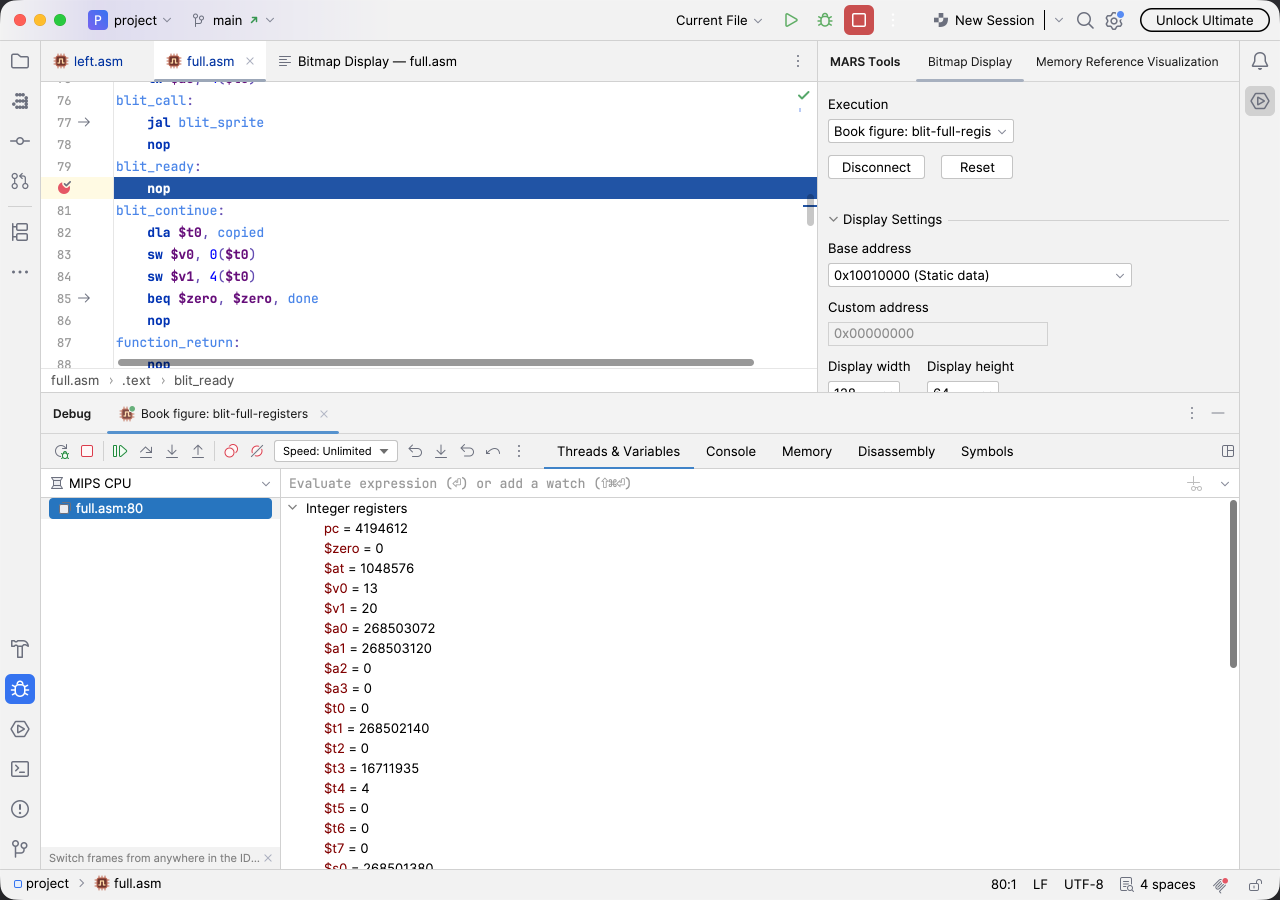
\includegraphics[artifact]{packages/016-clipped-sprite-blitter/captures/f02/registers.png}}
\sbox2{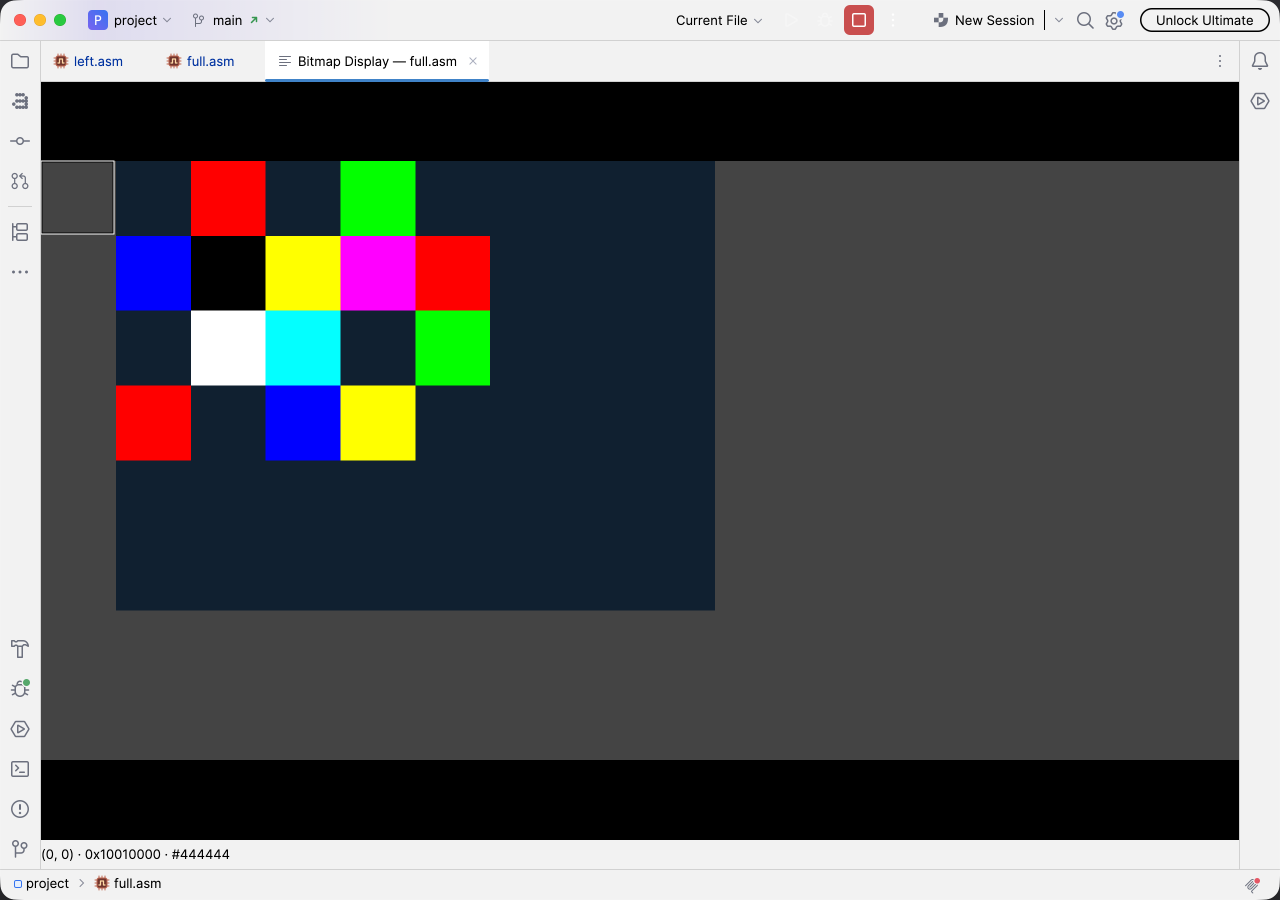
\includegraphics[artifact]{packages/016-clipped-sprite-blitter/captures/f02/bitmap.png}}
\sbox4{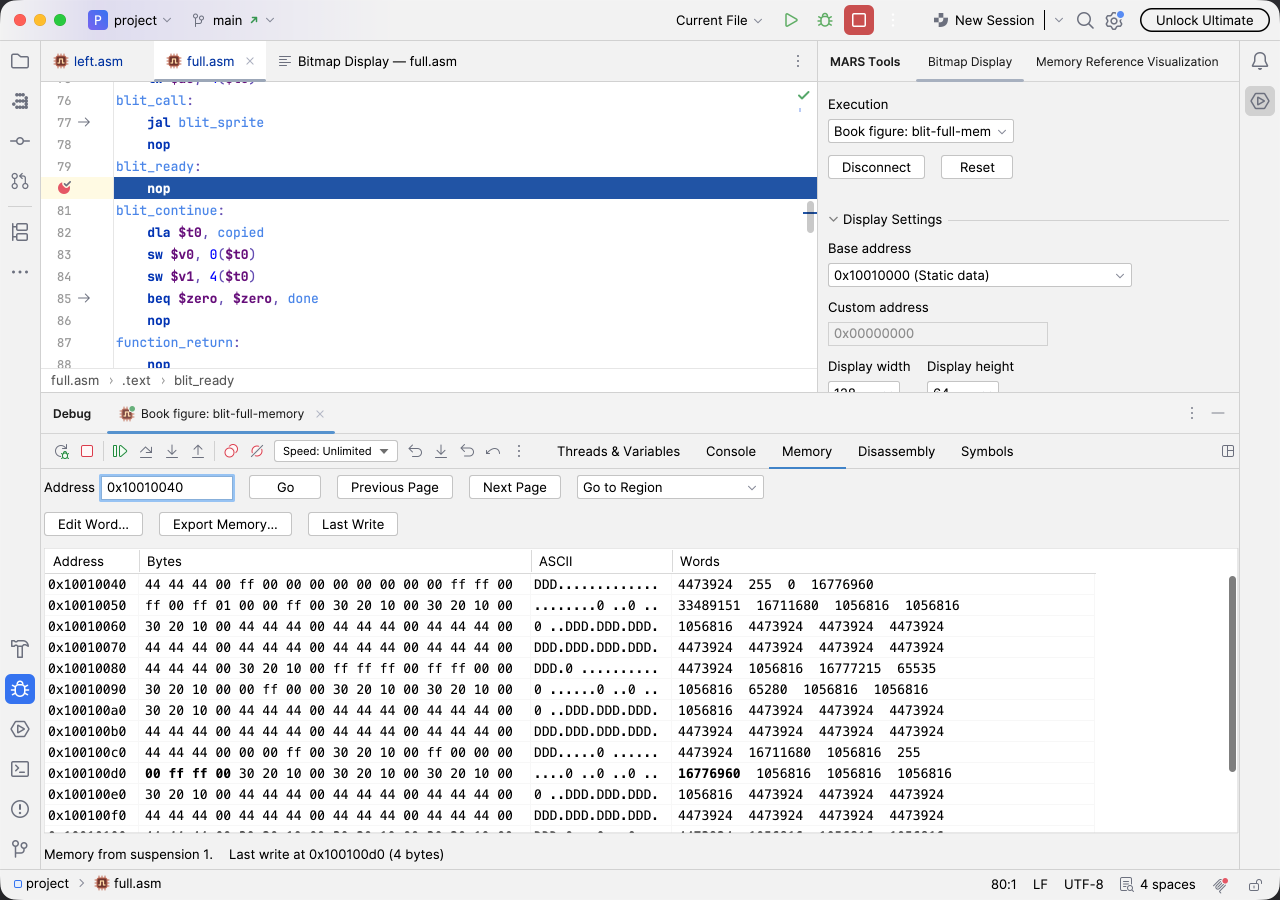
\includegraphics[artifact]{packages/016-clipped-sprite-blitter/captures/f02/memory.png}}
\edef\MARSblitfullsourceLeft{\the\dimexpr0.036718750\wd0\relax}
\edef\MARSblitfullsourceBottom{\the\dimexpr0.774444444\ht0\relax}
\edef\MARSblitfullsourceRight{\the\dimexpr0.713281250\wd0\relax}
\edef\MARSblitfullsourceTop{\the\dimexpr0.147777778\ht0\relax}
\edef\MARSblitfullregistersLeft{\the\dimexpr0.246093750\wd0\relax}
\edef\MARSblitfullregistersBottom{\the\dimexpr0.312222222\ht0\relax}
\edef\MARSblitfullregistersRight{\the\dimexpr0.553906250\wd0\relax}
\edef\MARSblitfullregistersTop{\the\dimexpr0.640000000\ht0\relax}
\edef\MARSblitfullbitmapLeft{\the\dimexpr0.032031250\wd2\relax}
\edef\MARSblitfullbitmapBottom{\the\dimexpr0.155555556\ht2\relax}
\edef\MARSblitfullbitmapRight{\the\dimexpr0.032031250\wd2\relax}
\edef\MARSblitfullbitmapTop{\the\dimexpr0.178888889\ht2\relax}
\edef\MARSblitfullmemoryLeft{\the\dimexpr0.034375000\wd4\relax}
\edef\MARSblitfullmemoryBottom{\the\dimexpr0.311111111\ht4\relax}
\edef\MARSblitfullmemoryRight{\the\dimexpr0.584375000\wd4\relax}
\edef\MARSblitfullmemoryTop{\the\dimexpr0.608888889\ht4\relax}
\begin{tikzpicture}[alt={Four annotated details after an unclipped five-by-four sprite copy. Return values are thirteen copied and twenty visible. The physical display starts with a guard before the eight-by-six logical framebuffer. A displayed magenta pixel is opaque because its stored word is 01ff00ff, which differs from the transparent key 00ff00ff. A memory detail at 0x10010050 shows bytes ff 00 ff 01.}]
\node[anchor=north west,inner sep=0,font=\small\bfseries] (source-title) at (6mm,0) {Next instruction after return};
\node[anchor=north west,inner sep=0] (source) at ([yshift=-1mm]source-title.south west) {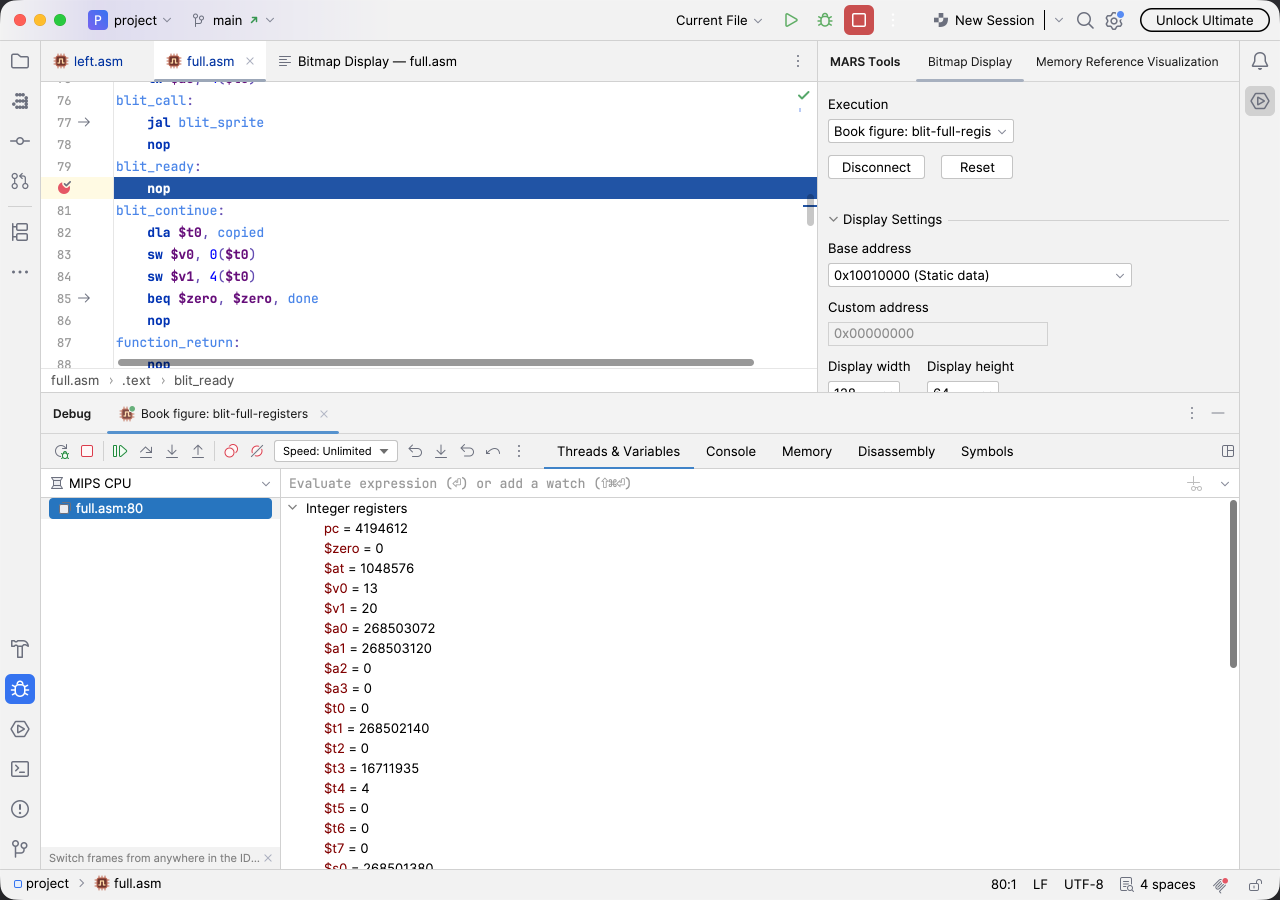
\includegraphics[width=0.54\linewidth,artifact,trim={\MARSblitfullsourceLeft{} \MARSblitfullsourceBottom{} \MARSblitfullsourceRight{} \MARSblitfullsourceTop{}},clip]{packages/016-clipped-sprite-blitter/captures/f02/registers.png}};
\begin{scope}[shift={(source.south west)},x={($(source.south east)-(source.south west)$)},y={($(source.north west)-(source.south west)$)}]
\draw[black,line width=0.7pt] (0.215625000,0.057142857) rectangle (0.384375000,0.371428571);
\node[draw=black,fill=white,circle,inner sep=1.5pt,font=\footnotesize] at ($(0.215625000,0.371428571)+(-3mm,0)$) {1};
\end{scope}
\node[anchor=north west,inner sep=0,font=\small\bfseries] (registers-title) at (0.58\linewidth,0 |- source-title.north) {Signed return values};
\node[anchor=north west,inner sep=0] (registers) at ([yshift=-1mm]registers-title.south west) {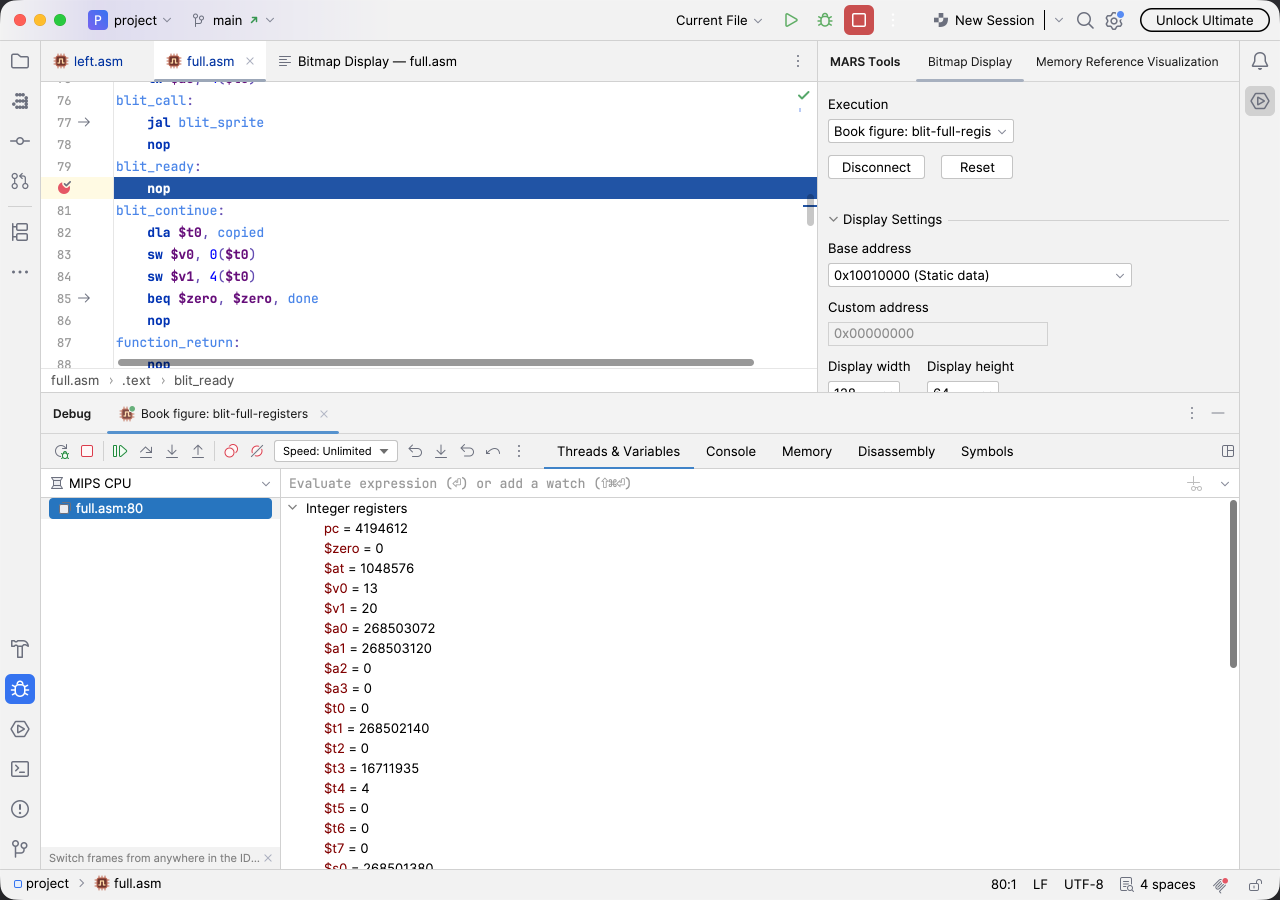
\includegraphics[width=0.42\linewidth,artifact,trim={\MARSblitfullregistersLeft{} \MARSblitfullregistersBottom{} \MARSblitfullregistersRight{} \MARSblitfullregistersTop{}},clip]{packages/016-clipped-sprite-blitter/captures/f02/registers.png}};
\begin{scope}[shift={(registers.south west)},x={($(registers.south east)-(registers.south west)$)},y={($(registers.north west)-(registers.south west)$)}]
\draw[black,line width=0.7pt] (0.023437500,0.023255814) rectangle (0.250000000,0.953488372);
\node[draw=black,fill=white,circle,inner sep=1.5pt,font=\footnotesize] at ($(0.023437500,0.953488372)+(-3mm,0)$) {2};
\end{scope}
\node[anchor=north west,inner sep=0,font=\small\bfseries] (bitmap-title) at ([yshift=-3mm]source.south west) {Complete physical Bitmap view};
\node[anchor=north west,inner sep=0] (bitmap) at ([yshift=-1mm]bitmap-title.south west) {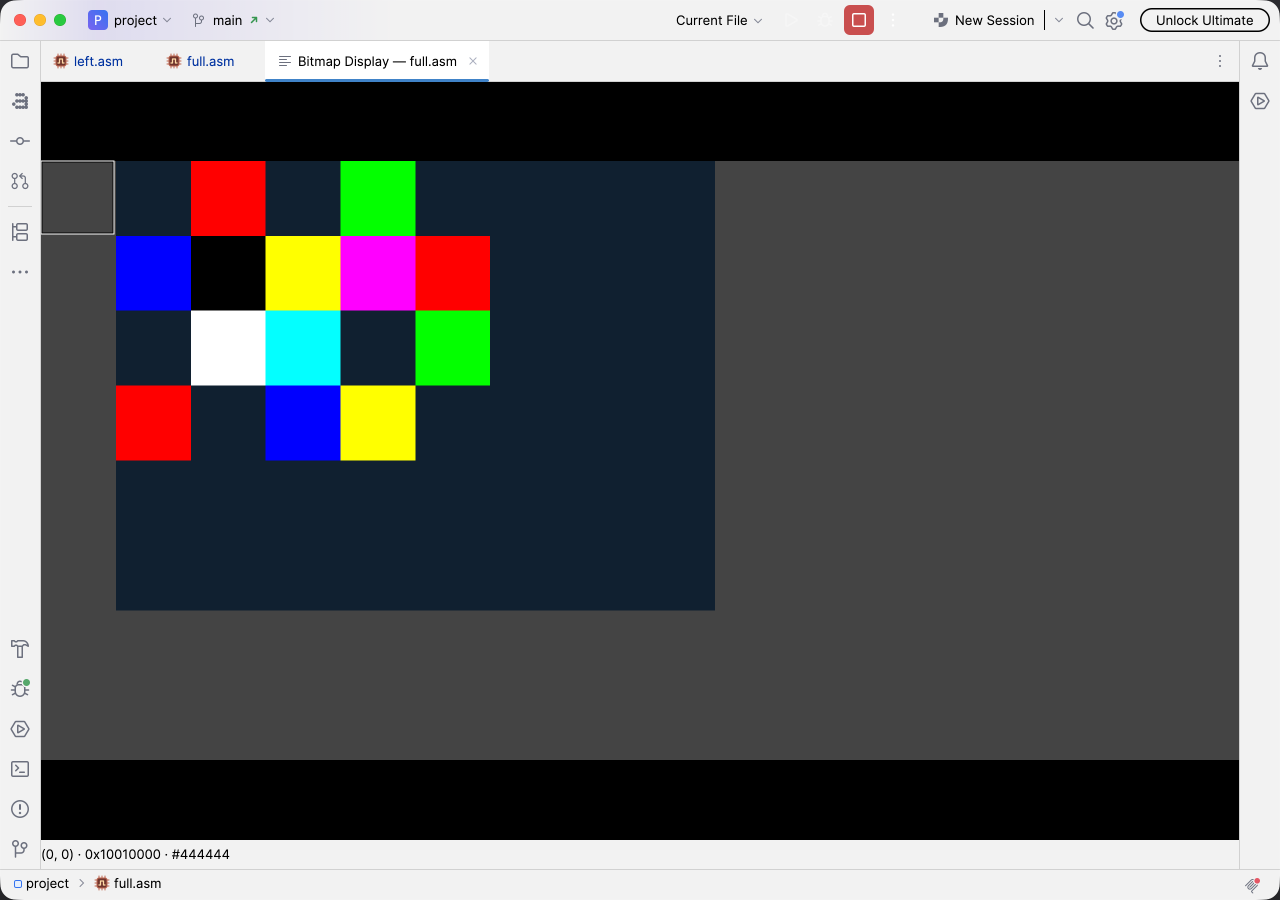
\includegraphics[width=0.56\linewidth,artifact,trim={\MARSblitfullbitmapLeft{} \MARSblitfullbitmapBottom{} \MARSblitfullbitmapRight{} \MARSblitfullbitmapTop{}},clip]{packages/016-clipped-sprite-blitter/captures/f02/bitmap.png}};
\begin{scope}[shift={(bitmap.south west)},x={($(bitmap.south east)-(bitmap.south west)$)},y={($(bitmap.north west)-(bitmap.south west)$)}]
\draw[black,line width=0.7pt] (0.000000000,0.000000000) rectangle (1.000000000,1.000000000);
\node[draw=black,fill=white,circle,inner sep=1.5pt,font=\footnotesize] at ($(0,1.000000000)+(-3mm,0)$) {3};
\draw[white,dashed,line width=0.7pt] (0.0625,0.25) rectangle (0.5625,1);
\end{scope}
\node[anchor=north west,inner sep=0,font=\small\bfseries] (memory-title) at ([yshift=-3mm]bitmap.south west) {Destination words, including neighboring padding};
\node[anchor=north west,inner sep=0] (memory) at ([yshift=-1mm]memory-title.south west) {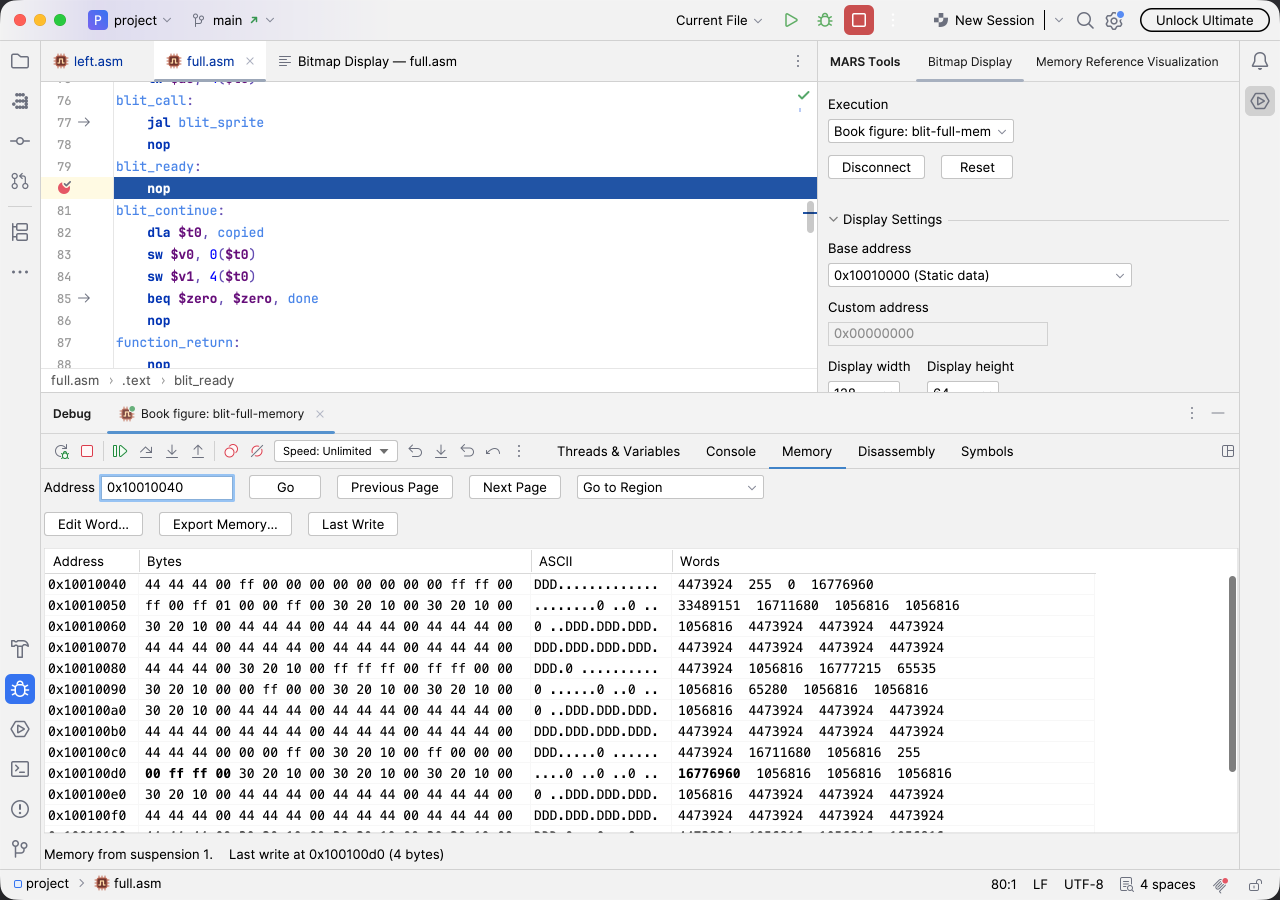
\includegraphics[width=0.84\linewidth,artifact,trim={\MARSblitfullmemoryLeft{} \MARSblitfullmemoryBottom{} \MARSblitfullmemoryRight{} \MARSblitfullmemoryTop{}},clip]{packages/016-clipped-sprite-blitter/captures/f02/memory.png}};
\begin{scope}[shift={(memory.south west)},x={($(memory.south east)-(memory.south west)$)},y={($(memory.north west)-(memory.south west)$)}]
\draw[black,line width=0.7pt] (0.194672131,0.055555556) rectangle (0.997950820,0.638888889);
\node[draw=black,fill=white,circle,inner sep=1.5pt,font=\footnotesize] at ($(0,0.638888889)+(-3mm,0)$) {4};
\end{scope}
\end{tikzpicture}
\par\smallskip
\begin{minipage}{\linewidth}
\small
\begin{enumerate}
\setlength{\itemsep}{2pt}
\setlength{\parsep}{0pt}
\item This fixture changes only the placement words to $(0,0)$. The next instruction at \texttt{blit\_ready} marks the completed image copy, before the caller publishes its two result words.
\item \texttt{\$v0 = 13} and \texttt{\$v1 = 20}. The entire five-column, four-row source rectangle fits within the eight-by-six frame. All twenty source words are examined. Seven equal the full transparent key and are skipped, leaving thirteen destination stores.
\item The image has sixteen physical columns and eight rows. Logical framebuffer cell $(0,0)$ is physical column 1, row 0, after the leading guard; each logical row has eight active cells and a sixteen-word stride. The dashed white outline marks the eight-by-six logical framebuffer. Gray cells include padding and the guard. The display omits the final padding word and trailing guard, which are checked separately in memory. The sprite occupies logical columns 0 through 4 and rows 0 through 3. Its black cell is a copied zero word, not an absent pixel. A magenta cell can also be copied: the display uses low RGB bits, while transparency compares the complete word.
\item Logical row 1 begins at \texttt{0x10010044}. Its first source values are blue, black, yellow, \texttt{0x01ff00ff}, and red. At \texttt{0x10010050}, bytes \texttt{ff 00 ff 01} encode that fourth word in little-endian order. It displays magenta but differs from key \texttt{0x00ff00ff} in its high byte, so it is opaque. Masking to RGB before the key comparison would incorrectly skip this cell and reduce the copied count.
\end{enumerate}
\end{minipage}
\caption{Placement $(0,0)$ examines all twenty sprite cells and copies thirteen full-word opaque pixels.}
\label{capture:016-clipped-sprite-blitter-f02}
\label{blit-f02}
\end{figure}
\par
